\documentclass[tikz, border=0 3pt 0 3pt]{standalone}

\begin{document}
 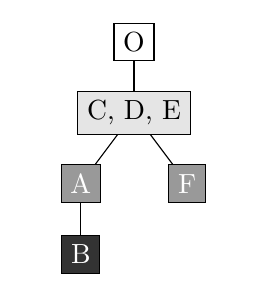
\begin{tikzpicture}[scale=0.9]
      \tikzset{every node/.style={draw=black, rectangle}}
      \path[use as bounding box] (-1.5,0.2) rectangle (1.5,-3.2);
      % \foreach \x in {0,1,...,3} {
      %   \draw[gray, dashed] (-1.5,-\x) -- (1.5,-\x);
      % }

      \node[fill=white] {O} [level distance=1cm]
      child { node[fill=black!10] {C, D, E}
        child { node[white,draw=black,fill=black!40] (A) {A}
          child { node[white,draw=black,fill=black!80] {B} }
        }
        child { node[white,draw=black,fill=black!40] {F} }
      }
      ;
    \end{tikzpicture}
\end{document}